%\begin{columns}[onlytextwidth]
%    \begin{column}{0.45\textwidth}
%        column
%    \end{column}
%    \begin{column}{0.45\textwidth}
%        column
%    \end{column}
%\end{columns}

\begin{frame}{The Cherenkov Telescope Array}
  \begin{columns}[onlytextwidth]
      \begin{column}{0.35\textwidth}
        \begin{itemize}
          \setlength\itemsep{1em}
          \item<1-> Open, proposal driven observatory
          \item<2-> 2 sites (CTA North and CTA South)
          \item<3-> 3 different telescopes (SST, MST, LST)
        \end{itemize}
      \end{column}
      \begin{column}{0.65\textwidth}
        \centering
        \only<2>{
          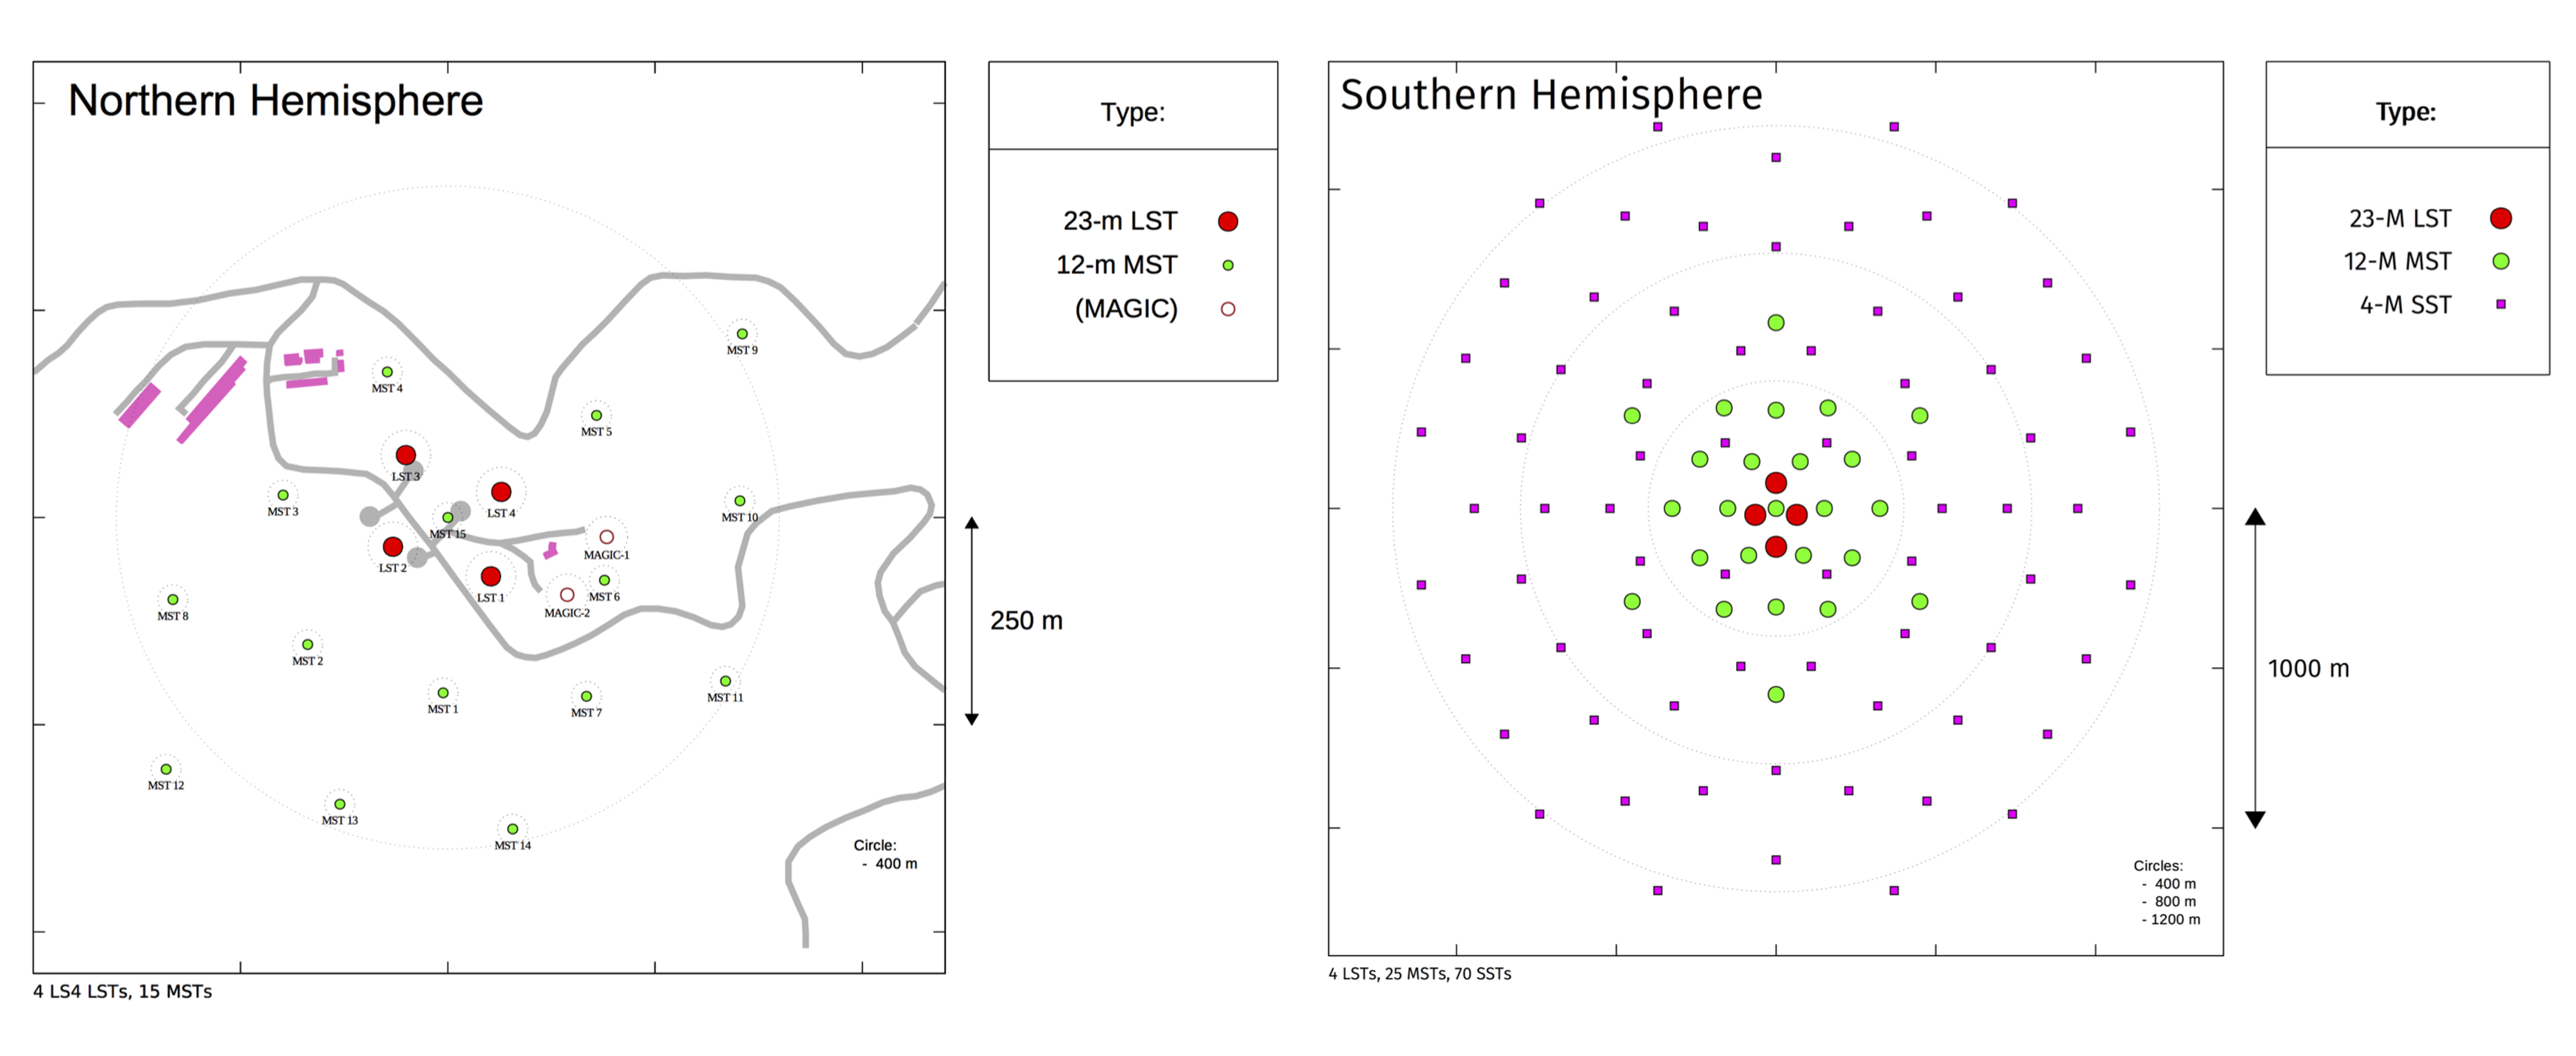
\includegraphics[width=\textwidth]{images/Array-Layouts.png}\\[-.75\baselineskip]
          \hspace{7cm}\small\href{https://www.cta-observatory.org/project/technology/}{[cta-observatory.org]}
        }
        \only<3>{
          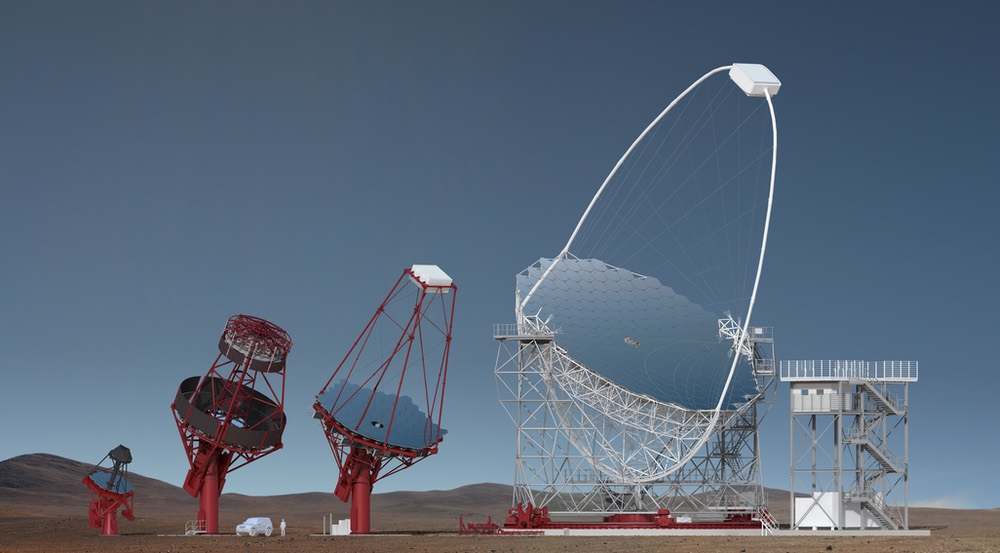
\includegraphics[width=0.9\textwidth]{images/telescopes.jpg}\\
          \hspace{6.75cm}\small\href{https://www.cta-observatory.org/project/technology/}{[cta-observatory.org]}
        }
      \end{column}
  \end{columns}

  \note<1->[item]{Öffentliches Observatorium (Daten jedem zugänglich)}
  \note<2->[item]{2 Standorte 
    \newline $\to$ Nörtliche Himmelsphäre: La Palma \& Südliche Himmelsphäre: Atacama Wüste, Chile
    \newline $\to$ Himmel vollständig abgedeckt
  }
  \note<3->[item]{Bestehen aus 3 verschiedenen Teleskopen $\to$ Bild}
\end{frame}

\begin{frame}{The LST-1 prototype}
  \begin{columns}[onlytextwidth]
    \begin{column}{0.5\textwidth}
      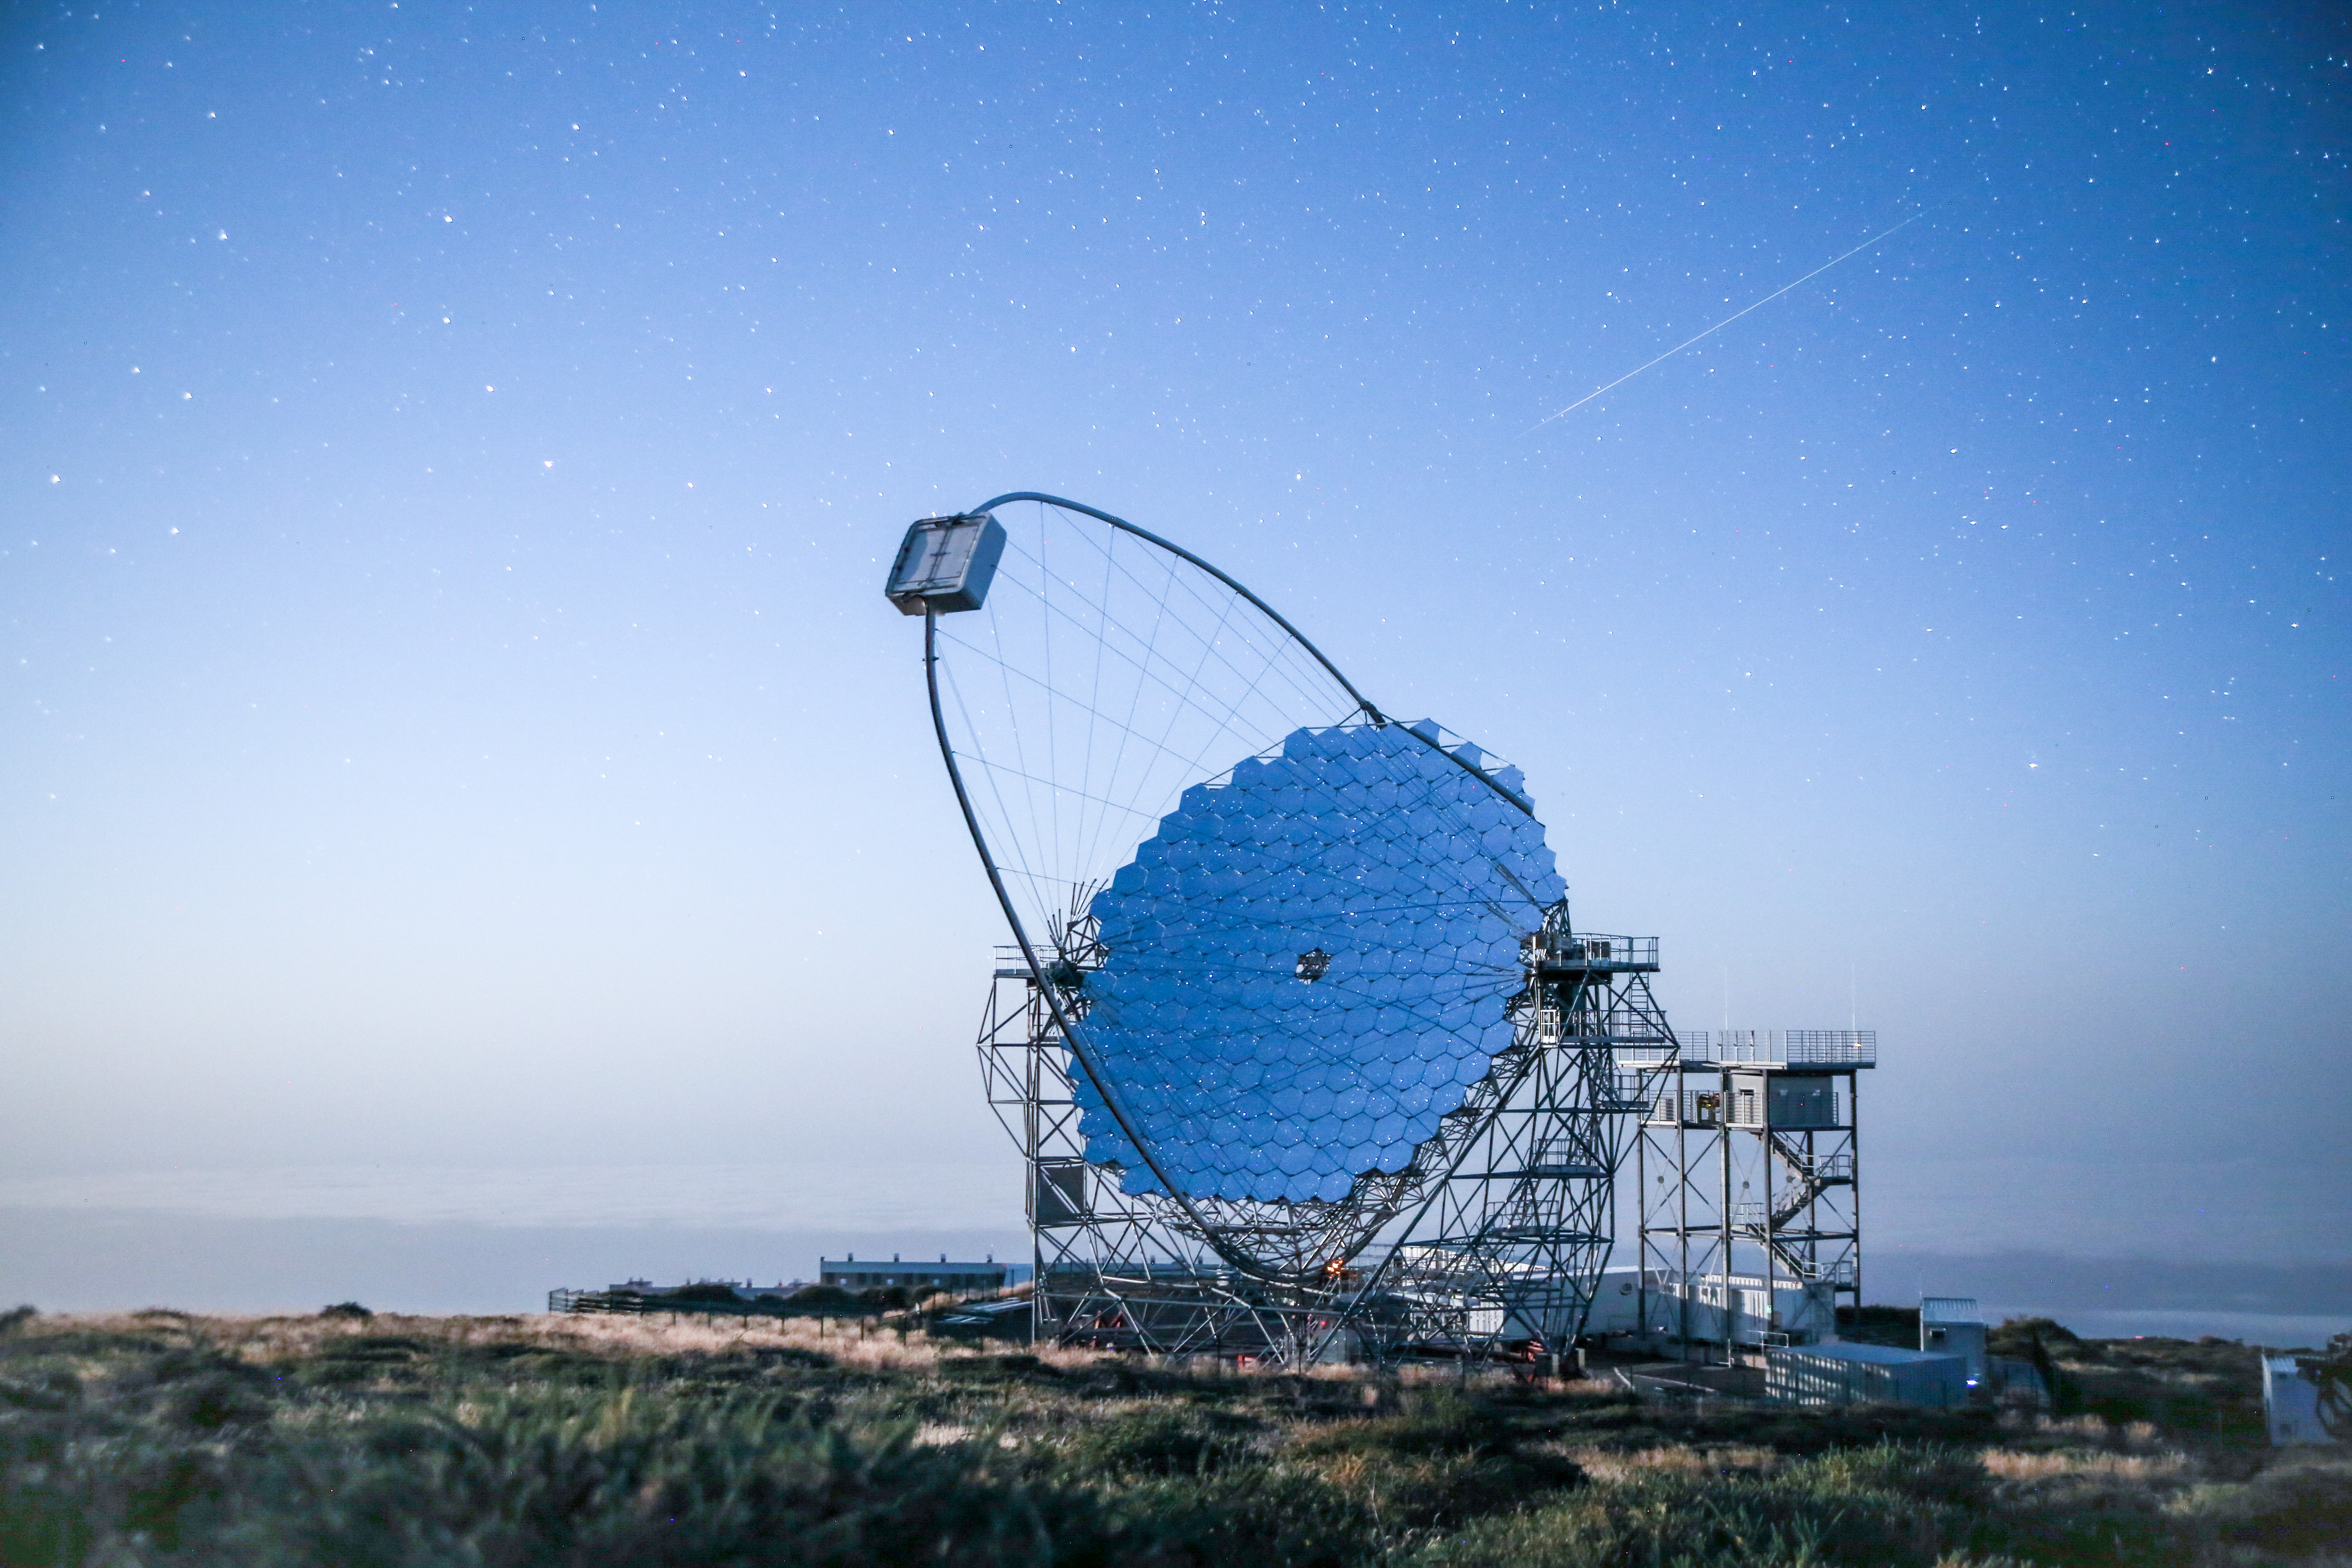
\includegraphics[width=\textwidth]{images/LST_1.jpg}\\
      \small\href{https://www.flickr.com/photos/cta_observatory/albums/72157671493684827/with/48629242378/}{[flickr.com/photos/cta\_observatory]}
    \end{column}
    \begin{column}{0.45\textwidth}
      \textcolor{tugreen}{Location:} Observatorio del Roque de los Muchachos, La Palma, Spain\\
      \textcolor{tugreen}{Mirror diameter:} \SI{23}{\meter}\\
      \textcolor{tugreen}{FOV:} \SI{4.3}{\degree}\\
      \textcolor{tugreen}{Camera:} \num{1855} pixel, photomultiplier tubes\\
      \medskip
      \textbf{\textcolor{tugreen}{\to}} Currently in commissioning phase
    \end{column}
  \end{columns}

  \note[item]{La Palma $\to$ Observatorio del Roque de los Muchachos}
  \note[item]{Spiegeldurchmesser = 23m}
  \note[item]{FOV = \SI{4.3}{\degree}}
  \note[item]{Kamera: \num{1855} pixel, photomultiplier tubes}
  \note[item]{Aktuell Testphase}
\end{frame}